\documentclass[openany,fontset=none]{intromech}


\begin{document}


% 封面

\includepdf{body/0.01-frontpage.pdf}

% 标题页
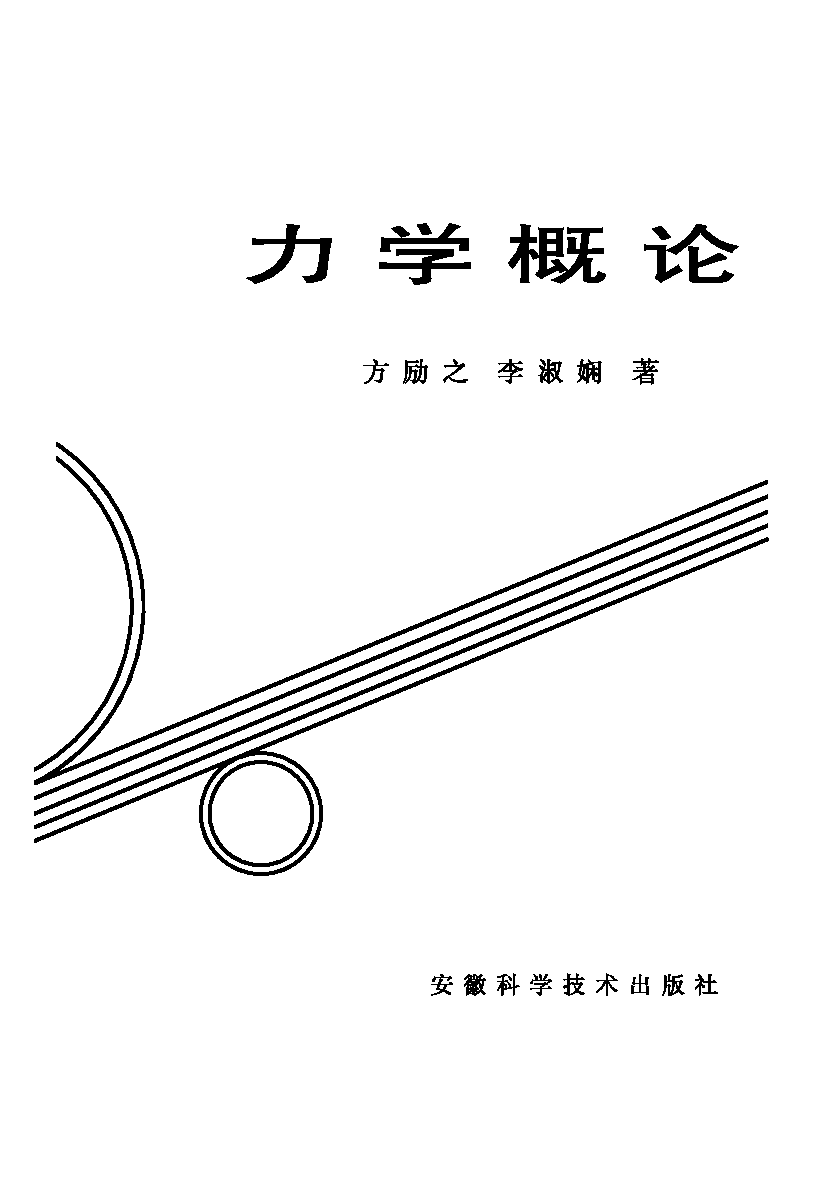
\includepdf{body/0.02-titlepage.pdf}

% 出版信息页
% 出版信息页
\begin{center}
    \zihao{4}\fangsong \mbox{}

    \mbox{}

    责任编辑:张晓红

    封面设计:陈治黄

    \vfill \heiti 力~~学~~概~~论

    \normalsize \kaishu 方励之~~李淑娴

    \normalfont *

    安徽科学技术出版社出版

    \zihao{-5} (合肥市跃进路1号)

    \normalsize 安徽省%
    \hspace{0.2em}\raisebox{-0.5mm}{
\includegraphics[width=4em]{icon/xinhuabokestore}}\hspace{0.2em}%
    发行~~安徽新华印刷厂印刷

    *

    \zihao{6}开本:850$\times$1168~~1/32~~印张:12.5~~字数:309,000

    1986年1月第一版~~~~1986年1月第一次印刷

    印数00,001—5,000

    \normalsize 统一书号:13200$\cdot$68~~~~定价:2.5元
\end{center}
\thispagestyle{empty}
\clearpage


% 内容提要
% 内容提要
\begin{center}\begin{minipage}{8.4cm}\vspace{3cm}
        \begin{center}\heiti 内~容~提~要\end{center}
        \normalfont \zihao{-5}
        \hspace{2em}本书是根据作者在中国科学技术大学及北京大学讲授普通物理的
        力学部分讲稿整理而成的。其特点是强调用物理的前沿发展去改进基础物理教
        学,即用现代物理的观点去选择课程的内容,去表现概念和规律。因此,书中
        包括一些在传统的教材中没有的内容,如牛顿宇宙学等,对许多传统的内容,
        也采取新的讲授法,使之能与当代物理的进展相呼应。另外。由于力学是物理
        学的入门和基础,所以本书也注意物理方法的阐述,这对于初学物理的学生是
        有益的。书中还附有一些习题及答案。

        \hspace{2em}本书可作为综合大学及师范院校的普通物理力学教材,也可供大
        专院校物理教师及物理教学研究工作者参考。
\end{minipage}\end{center}
\thispagestyle{empty}
\clearpage

% 序言
\setcounter{page}{1}
\pagestyle{foreword}
\null\vspace{1em}
\begin{center}
    \zihao{4}\heiti 序

    \null
\end{center}
\fangsong \normalsize

这本书原是一份普通物理课程的力学讲义,它曾在中国科学
技术大学沿用多年,也曾在北京大学教授过数次。

    普通物理中的力学,是相当难教的,凡是教授过这门课的老
师,大都有此体会。一方面,力学是整个物理学的基石,它包含
许多基本的观念、方法和理论,需要学生极为准确地加以掌握,
以备后继学习之用,另一方面,初入大学的学生,往往看轻力学,
误认为新的内容不多,似乎在中学里都已学过,结果力学反而被
疏忽了。

    这种局面迫使一些教师采用理论力学的方法来教授普通物理
力学。这样做,确实可以解决前述问题的第二方面,学生不再感
到“似曾相识”了。随着教和学二者的提高,原属理论力学的部
分内容的确可以逐渐放到普通物理中来。但是,我们觉得,若仅
限于这一途径改进教学,还不能或不完全能解决问题的第一个方
面——力学是整个物理的一块基石。

    基石到底在哪里起了基石的作用?基石到底如何起了基石的
作用?显然,这些“哪里”,这些“如何”只有从物理的当代发
展以及前沿研究的角度,才能看得清楚。这就是说,如果我们企图
从“物理的基石”这一标准来组织教学,它至少有以下两方面的
含义:一是不断用新的现代的观点去整理老的内容,一是不断用新
的前沿的重要成果来充实基础。事实上,不同时代的教材的差别,
最清楚地表现在这些方面。上进的标准,也就是我们在编写这本
教材时,尝试着击追求的。也许有的地方达到了,也许有的地方%分页处
并未达到。无论成功或失败,它都是我们的追求的记录。

为了使用上的方便,书中编辑了一些例题,每章末也附有一
些思考题和习题。由于北京大学物理系和中国科学技术大学物理
教研室已编有《物理学习题集》(人民教育出版社,1980),为了不
重复太多,本书中的例题和习题只是标志性的。在教学上需要更
多习题时,可以参考上述的习题集。

在使讲义变成这本书的过程中,得到过员汝槐同志的协助,
谨致谢意.

~

\hspace{6.8cm}\zihao{-4}\kaishu 作~~~者

\mbox{}

\hspace{7cm}\normalfont \zihao{-5}1984年4月\normalsize
\clearpage

% 目录
\clearpage
\setcounter{page}{1}
\tableofcontents

% 正文
\clearpage
\pagestyle{heading}
\setcounter{page}{1}
% 公式与上下文本距离调整
\setlength\abovedisplayskip{1pt plus 3pt minus 7pt}
\setlength\belowdisplayskip{1pt plus 3pt minus 7pt}

% 绪论
\ichapter{——物理世界的统一}

物理学的兴起,是从经典力学开始的。在经典力学之前,人类
的文明中虽然已有不少具有物理价值的发现和发明,但是并不存
在一门独立的物理学。因此,我们在学习经典力学的时候,首先
应当了解:为什么经典力学成了物理学的起点?经典力学在整个
物理学中占据着怎样的地位?

爱因斯坦曾经这样来概括牛顿力学的历史地位;“古代希腊
伟大的唯物主义者坚持主张,一切物质事件都应当归结为一系列
的有规律的原子运动,而不允许把任何生物的意志作为独立的原
因。而且无疑笛卡尔曾按他自己的方式重新探索过这一问题。但
是,在当时,它始终不过是一个大胆的奢望,一个哲学学派的成
问题的理想而已。在牛顿之前,还没有什么实际的结果来支持那
种认为物理因果关系有完整链条的信念。”

这句话的意思是,物理学依赖于一种基本的信念:物理世界
存在着完整的因果链条,即自然界是统一的。牛顿力学则是体现
这种信念的第一个成功的范例。

从牛顿力学的创建到现在,已经有三百多年了,物理学已经
大大发展了,远远超过了经典力学原有的水平。但是,就物理学
的最基本的追求和物理学的总目标来说,却一直没有变化。经典
力学时代的追求和目标,可以说时至今日仍然是整个物理学的追
求和目标。这个最基本的追求和目标,就是自然界的统一。的确,
从整个物理学的发展中,可以看到一条鲜明的主线。这就是执着%分页点
地追求宇宙的统一,找寻支配宇宙万物的最基本最统一的规律。

相信存在统一,努力寻求统一,如果仅仅作为一种自然观,
早在古代已经有了。老子的《道德经》中写有:“道生一、一生
二、二生三、三生万物。”这就是中国古代的一种统一观,它完
全可以与爱因斯坦所提及的古希腊的哲学相媲美。不过,无论在
古代中国或古希腊,统一观都只是一种哲学思辨。

牛顿的力学和古代的哲学不同,它不是思辨地坚持统一观,
而是发展了寻找统一的有效的物理方法。牛顿在他的最重要的力
学著作《自然哲学的数学原理》中阐明了他采用的方法。他在前
言中写道;“我奉献这一作品。作为哲学的数学原理,因为哲学
的全部责任似乎在于——从运动的现象去研究自然界中的力,然
后从这些力去说明其他的现象。”\sbfootnote{牛顿这段话里的
    “哲学”一词,实际含义相当于今天的“科学”或“物理学”。}这就是
说,寻求统一的出发点不是思辨而应是运动现象。自然界中的运动
现象是多种多样的,物理学的责任就在于寻找支配这些现象的统一的力。

今天的物理学,仍然大体地沿袭着牛顿所开创的研究途径。
寻找统一的力,或统一的相互作用。因此,几乎所有基本的物理
理论都称做某种力学,如牛顿力学、电动力学、色动力学等等。
每一种新的力学的确立,都标志着我们在追求统一的逾程上达到
了一个新的水平。

为了更具体地表达上述的论述。我们利用表1。表1左边列举
的是自然界中的种种运动现象,也就是物理学的研究对象。天体
的运行和地面物体的运动是人首先看到或接触到的,随后才有时
间、空间的概念,所以时空也是一种物理研究的对象,另一类现
象是电、磁和光,所有这些物理对象。在二十世纪之前,人们都
已知道了。二十世纪以来,又逐渐证实或发现一些新的对象。如
原予、原子核、核子以及夸克等。

表\ref{tab:1.00-01}~的其余部分就表示物理学在寻求统一,寻求完整的因果
链条上一些重要的阶段。
牛顿的力学和万有引力定律,是物理学上第一次大的统一。
在牛顿之前,传统的观念认为支配天体运行和支配地面物体运动
的规律是不相同的,有所谓天界和世俗两个世界之分。然而,牛
顿发现,天上行星和月亮的运动,实际上和地面落体运动遵从相
同的规律,它们都是由引力引起的。这样,牛顿就用他的力学打
破了天界和世俗的界限,找到了两个世界的统一。牛顿称引力为
万有引力,就是强调这种统一。

第二次大的统一,是由十九世纪的麦克斯韦完成的。他建立
了电磁理论,使电、磁及光学现象得到统一。这就是电动力学。

很快发现,牛顿的力学和麦克斯韦的电磁学这两大领域在时
\begin{table}[!h]
    \centering
        \vspace{-0.5em}
        \caption{物理学发展中的统一}
        \label{tab:1.00-01}
        \begin{tabular}{c}
            \toprule \vspace{-1em} \\
        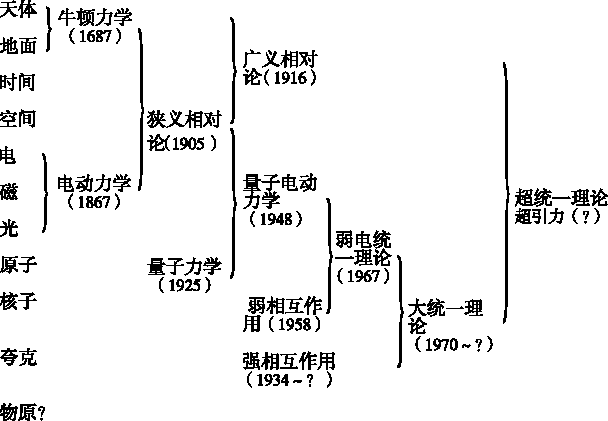
\includegraphics[width=0.98\linewidth]{figure/1.00-tab01}\\
        \bottomrule
        \zihao{6}* 括号中的数字表示相应的理论建立的年代;有问号的表示尚未完成。
        \end{tabular}
\vspace{-1.2em}
\end{table}
空观上是很不协调的。在前者中,各种匀速运动是平权的,但却
假定有绝对空间或绝对速度存在。相反,在后者中,有一个地位
特殊的速度,即光速,但却始终测不出这个特殊的速度是相对于
哪一个绝对空间而言的。爱因斯坦抛弃了绝对空间观念,使电磁
学、力学在新的时空观的基础上达到了协调和统一。

爱因斯坦还曾企图把引力和电磁力二者统一起来,但他的努
力没有成功。然而,他却找到了能与麦克斯韦电磁理论相协调的
引力理论——广义相对论。

作为引力理论的广义相对论和作为电磁理论的麦克斯韦理论
构成了我们今夭称为经典物理学的理论基础。

与经典物理相对的是量子论。量子力学最初是作为原子、分
子的统一的力学而发展起来的。这种新的力学统一地解释了原子、
分子的各种光谱现象,统一地解释了元素周期表,统一地解释了
各种不同分子的键合。

在将量子力学扩展到电磁场时,遇到了困难,这本质上是由
于电磁场是相对论性的。直到四十年代末,发展了所谓重整化方
法才巧妙地解决了上述的困难,使量子论与电磁理论能得以统一,
产生了量子电动力学。

到六十年代末,我们已经得到了如下的物理世界的图象。宇
宙中的所有物理对象可以分成两大类,一类称为“物质”,如夸
克、电子、$\mu$子等等,另一类称为“相互作用”,如引力、电磁力
等等。在目前的宇宙中,有四种基本的相互作用,按它们的强度
顺序排列是:核子参与的强相互作用,荷电粒子参与的电磁相互
作用,核子及电子、中微子参与的弱相互作用,以及任何粒子都
参与的引力相互作用。可以简单地说,宇宙间的一切运动和变化。
都可以统一为这四种“力”的作用。但是,追求统一的物理学,
似乎认为这种状况仍然不够统一。

1967年,温伯格和萨拉姆再次着眼于统一,先后提出了电磁
相互作用和弱相互作用的统一理论。随后的一系列实验证明他们
的统一理论是正确的。

这一新的成功,促使许多人去找寻把电磁作用、弱作用及强
作用都包含在内的统一理论,通常称为“大统一理论”。建立这
种理论的工作还没有完成,这是正在研究的领域。

如果大统一能够顺利完成,下一步的统一就是要把引力也统
一在内了。引力是物理学最早讨论的一种基本的力。但是,它与
其他力的统一最难,因为引力有一系列很特别的性质。例如这种
力只有引力却无斥力。就是这种特别性质之一。

企图把引力与其他力统一起来的工作,称为超统一的研究。
目前还没有得到有实际意义的结果。它是今天的物理学的一个前
沿。实现超统一的一个可能是用超引力理论,这种理论中的统一
有一个很有趣的特点,即它把物理学中传统的“物质”与“相互
作用”之间的界限也打破了。

总之,从牛顿力学开始,物理学就在寻找宇宙的统一,我们
希望找到控制着万事万物运动的极少的几个基点。只有从这个角
度我们才容易看清经典力学在整个物理学中的地位和作用,也才
能全面地了解学习经典力学对于学习整个物理学的意义和作用。


% 第一章
\chapter{时间,空间和运动学}

\section[时间]{时~~~~间}
描写物体的运砖。要用时间和空间这两个概念.因此,我们
先来对时间,空间本身作一些分析。

时间和空间可以说是最平凡的概念了,因为在日常生活中也
常常用到它们。不过,若问什么是时间?什么是空间?却又不容易
找到恰当的答案。其实,这是两个很难的问题.尽管有不少关于
时间和空间的定义,但大都不能令人满意。一种或许可以接受的
说法是:时间、空间是物理事件之间的一种次序,时间用以表述
事物之同的顺序,空间用以表述事件相互之间的位形。

没有满意的“严格”的理论定义,并不妨碍时间和空间二者
在物理中的使用。因为,物理学是一门基于实验的科学,在考查
物理学的概念或物理量的时候,首先应当注意它与实验之间是否
有明确的、不含糊的关系。对于时间和空间这两个基本概念来说,
首要的问题似不是去追究它们的“纯粹”定义,而是应当了解它
们是怎样量度的。

量度时间,通常是用钟和表。然而,钟和表并不是测量时间
的唯一的工具。原则上。任何具有重复性的过程或现象,都可以
作为测量时间的一种钟。自然界里有许多重复性的过程,其中有
一些我们早已把它们当作计时标准了。例如,太阳的升没表示天;
四季的循环称作年;月亮的盈亏是农历的月。其他的循环过程,
如双星的旋转、人体的脉搏、吊灯的摆动,分子的振动等等,也
都可以用作测时的工具。

更一般地说,只要知道了某个物理现象随时问的变化,尽管
它不是重复性的过程,也可以用来测定时间。譬如,我们能从一
个人的容貌估计出他的年龄,因为容貌这个量与时间之间有确定
的关系。这个例子虽然很普通,但某些有用的测时方法与此是很
相似的。在确定星体的年龄时,常常就是根据星体的颜色。

钟的种类很多,但有好有坏。比较两个人的脉搏,就会发现
它们之间经常有明显的快慢波动,所以,人的脉搏不是一种好钟,
它不够稳定。如果比较一下两个单摆的周期,就会发现它们稳定
多了。地球自转则是更稳定的钟。
\begin{figure}[!h]
    \centering
    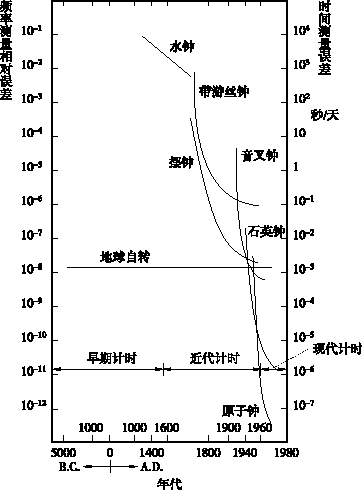
\includegraphics[height=8cm]{figure/1.01-fig01}
    \caption{不同年代的时间测量精度}
    \label{fig:1.01-01}
\end{figure}

图\ref{fig:1.01-01}~给出不同年代用不同的钟测量时间所达到的精度。可以
看到,地球自转要比各种机械的钟都好。所以,1967年以前是用
地球自转作为标准钟。原子钟是比地球自转更加稳定的钟,现代
的精密计时都是用原子钟了。

\begin{table}[!h]
    \centering
    \vspace{-0.5em}
    \caption{一些典型物理现象的时间尺度}
    \label{tab:1.01-01}
    \begin{tabular}{c}
        \toprule \vspace{-1em} \\
        
\includegraphics[width=0.8\linewidth]{figure/1.01-tab01}\\
        \bottomrule
    \end{tabular}
    \vspace{-1.2em}
\end{table}
\clearpage
    1967年10月在第十三届国际度量衡会议上通过了新的标准
钟,它对一秒的时间作如下的规定;位于海平面上的$^{133}$Cs原子
的基态的两个超精细能级在零磁场中跃迁辐射的周期$T$与1秒的
关系为

\centerline{1秒=9,192,631,770$T$}

表\ref{tab:1.01-01}~列举了一些典型现象的时间尺度。目前,物理学中涉及
的最长的时间是:\num{e38}秒,它是质子寿命的下限。宇宙的年龄大约
是\num{6e17}秒,即200亿年。牛顿力学所涉及的时问尺度大约是
\num{e-3}~\num{e15}秒,即从声振动的周期到太阳绕银河中心转动的周期。
粒子物理的时间尺度都很小。$\mu$子的寿命是\num{2e-6}秒。已经算是
极长寿的了。最短寿的是一些共振粒子,它们的寿命只约有\num{e-24}
秒。目前物理学中涉及的最小的时间是\num{e-42}秒,称为普朗克时
间。普朗克时间被认为是最小的时间,比普朗克时间还要小的范
围内,时间的概念可能就不再适用了。
\section{芝诺佯谬和时间的度量}
古希腊哲学家芝诺有一个很著名的论证:跑得最快的神话英
雄阿基里斯是永远追不上跑得最慢的东西(例如一只龟)的。他的
论证如下:因为开始时阿基里斯是在龟的后面,所以,阿基里斯
要追上龟,他必定先要到达龟的出发点,这要用有限的时间,在
这段时间里龟必定向前跑了,到达前面的一点,而当阿基里斯再
到达这点时,龟必定又已到达更前面的一点。如此重复下去,就
是进行无穷多次,龟也总不舍落在阿基里斯之后。

这个论证被称为芝诺佯谬,如何解开这个佯谬?

关键是在芝诺佯谬中用了两种不同的时间度量。按上节的讨
论,任何一种具有重复性的过程。都可以做为“钟”,用其重复
的次数来量度时间。芝诺问题中。除了“普通”钟所测得的时间
$t$,还利用了一种很特别的钟,该钟使用的重复性过程是。阿基里
斯逐次地到达龟在前一次的出发点。我们称这种钟叫芝诺钟,它
测得的时间为$t'$。

\begin{figure}[!h]
    \centering
    \vspace{-0.5em}
    \import{figure}{1.01-fig02.pdf_tex}
    \caption{芝诺时的定义}
    \label{fig:1.01-02}
    \vspace{-1.2em}
\end{figure}
如图\ref{fig:1.01-02},阿基里斯和龟在开始时相距为$L$,速度分别为$v_1$及
$v_2$,并且$v_1>v_2$。如果用普通的钟,则阿基里斯将在
\begin{equation}
    t=L/(v_1-v_2)
    \label{equ:1.01.02-01}
\end{equation}
时,赶上龟;当$t>L/(v_1-v_2)$时,阿基里斯就超过龟了。

图中左边的数字表示的是芝诺时$t'$。当$t'=1$时,阿基里斯到
达龟在0时的出发点;当$t'=2$时,阿基里斯到达龟在1时的出发
点。一般地,当$t'=n$时,阿基里斯到达龟在$t'=n-1$时的位置。
显然,只有当$t'\rightarrow\infty$时,阿基里斯才能逼近龟,对于任何有限的
$t'$,阿基里斯总是落在龟的后面。这就是芝诺的结论。

因此,芝诺断言:“阿基里斯永远也追不上龟。”这里“永
远”的含意是$t'\rightarrow\infty$。,即芝诺时间的无限。

现在我们来讨论普通时$t$与芝诺时$t'$之间的变换关系。不难
验证表\ref{tab:1.01-02}~给出的两种时间的对应。因此,一般有
\begin{equation}
    t=\sum_{n=0}^{t^{\prime}-1} \frac{L}{v_{1}}\left(\frac{v_{2}}{v_{1}}\right)^{n}=\frac{L}{v_{1}-v_{2}}\left[1-\left(\frac{v_{2}}{v_{1}}\right)^{t'}\right]
    \label{equ:1.01.02-02}
\end{equation}%
或者\vspace{-1.2em}
\begin{equation}
    t^{\prime}=\frac{1}{\ln \left(v_{2} / v_{1}\right)} \ln \left[1-\left(\frac{v_{1}-v_{2}}{L}\right) t\right]
    \label{equ:1.01.02-03}
\end{equation}%
式(\ref{equ:1.01.02-02})或式(\ref{equ:1.01.02-03})称为芝诺变换。它给出的$t'$与t的关系。在
图1·3中画出。

\begin{table}[!h]
    \centering
    \vspace{-0.5em}
    \caption{普通时与芝诺时的关系}
    \label{tab:1.01-02}
    \begin{tabular}{c|l}
        \toprule
        芝诺时($t'$)& \hspace{7em}普通时($t$)\\
        \midrule
        0 & \qquad 0 \\
        \addlinespace
        1 & \qquad $\dfrac{L}{v_1}$  \\
        \addlinespace
        %\specialrule{0em}{3pt}{3pt}
        2 & \qquad $\dfrac{L}{v_1} + \dfrac{L}{v_1}\cdot\dfrac{v_2}{v_1}$ \\
        \addlinespace
        \vdots & \qquad \vdots \\
        \addlinespace
        $n$ & \qquad $\dfrac{L}{v_1} + \dfrac{L}{v_1}\cdot\dfrac{v_2}{v_1} + \dots + \dfrac{L}{v_1}\cdot(\dfrac{v_2}{v_1})^{n-1} $ \qquad \null\\
        \bottomrule
    \end{tabular}
    \vspace{-1.2em}
\end{table}
由图\ref{fig:1.01-03}~看到,芝诺变换是有奇性的,即当$t=L/(v_1-v_2)$时,
$t'\rightarrow\infty$。所以,当芝诺时$t'$从零变化到无限时,它只覆盖了普通时
$t$上的一个有限范围,即从零到$ L/(v_1-v_2) $。

因此,芝诺佯谬之“佯”,是由于芝诺把永远理解为$t'\rightarrow\infty$。
他认为$t'\rightarrow\infty$之后就没有时间了,故$t'\rightarrow\infty$相当于永远。实际上,
从图\ref{fig:1.01-03}看到,在芝诺时$ t' $到达无限之后。还是有时间的。但是,
在该范围,即$ t>L/(v_1-v_2) $,用芝诺钟已经无法度量它们了。简
言之,芝诺的佯谬,来源于芝诺时的局限性,芝诺时不可能度量
阿基里斯追上龟之后的现象。

芝诺佯谬给我们的启示是,时间与时间的度量不同,一种时\clearpage
\begin{wrapfigure}[10]{10}{48mm}
%    \vspace{-0.5em}
    \import{figure}{1.01-fig03.pdf_tex}
    \caption{芝诺时的定义}
    \label{fig:1.01-03}
    %\vspace{-1.2em}
\end{wrapfigure}
\noindent 间的度量达到无限之后,还是可以有时间的;反之,一种时
间的度量达到无限,从其他的度量看,可能是有限的。

芝诺佯谬还启发我们提出一个更深入的问题,即所谓普通钟
或日常钟是否也具有芝诺钟那种局限性?当日常钟$t$的读数达到
无限之后,是否也还有时间?是否有$t$也无法度量的现象,即在
$t\rightarrow\infty$之外的现象?现代物理学的研究,对这些
问题的回答都是肯定的。

\section[长度]{长~~~~度}
长度是空间的一个基本性质。

对长度的测量,在日常的范围中,是用各种各样的尺,如米
尺、千分尺、螺旋测微计等等。对于不能用尺直接加以测量的小
尺度,可以求助于光学方法。在精密机床上常有光学测量装置;
测定胰岛索中原子的位置,是用X衍射方法。对于大的尺度,
也不能直接用尺去测量,也要求助于光。测量月亮与地球的距离
可以用激光测距的方法;测量一些不太远的恒星,可以用三角学
方法,利用恒星发出的光。至于银河系之外的遥远天体的距离,
同样是用它们发光的一些特征来测定的。

最近,长度的单位和标准,也用光来规定了。

长度的位单是米。1960年以前,用铂铱米尺作为标准尺,规
定米的大小。1960年以后,改用光的波长作为标准。在第十一届
国际计量大会上,正式通过的“米”的定义是l米等于$^{86}$Kr原子
的$2p_{10}$和\proofnote{$5d_5$}{原文误作“$6d_5$”。}~能级之间跃迁时所对应的辐射在真空中的波长$\lambda$的l,650,763.73倍,即

\centerline{1米=l,650,763.73$\lambda$}

\renewcommand{\hsp}{\hspace{0.6em}}
1983\hsp 年\hsp 10\hsp 月召开的第十七届国际计量大会上已正式通过
\\
\begin{table}[!h]
    \centering
    \vspace{-0.5em}
    \caption{一些典型物理现象的空间尺度}
    \label{tab:1.01-03}
    \begin{tabular}{c}
        \toprule \vspace{-1em} \\
        
\includegraphics{figure/1.01-tab03}\\
        \bottomrule
    \end{tabular}
    \vspace{-1.2em}
\end{table}
\clearpage
\noindent 了新的米的定义,即用光速值来定义“米”,以代替1960年的规定。
新的米的定义是,米是光在真空中在1,299,792,458秒的时间间隔
内所传播的路程长度。按这种新的定义,光速c是一固定的常数,
即

\centerline{$c$=299,792,458米/秒}

表\ref{tab:1.01-03}~中列举了一些典型现象的空间尺度。目前,物理学中涉
及的最太长度是$10^{28}$米,它是宇宙曲率半径的下限;已达到的最
小长度为$10^{-20}$米,它是弱电统一的特征尺度。普朗克长度约为
$10^{-35}$米,被认为是最小的长度,意思是说,在比普朗克长度更小
的范围内,长度的概念可能就不再适用了。

\section[参考系]{参~~考~~系}
    牛顿力学所研究的对象是物体的机械运动。从我们日常见到
的车行马跑,及至大到月亮、太阳等星体的运行,小到分子、原子、
粒子的一些飞行,都是属于这一类运动。这类运动的共同特点,
就是物体在空间的位置时刻在变化着。当然,静止的状态、平衡
的状态也是力学的内容之一。

    牛顿意义下的运动学,就是研究如何描写物体位置的变化。

\renewcommand{\hsp}{\hspace{0.1em}}
    研究问题总是从简单的情况入手。我们首先讨论一种被称为
质点的物体,即大小为零的物体。我们知道,任何具体的物体总
是有一定大小的,没有任何一个物体与质点完全等价。但是,对
于某些特定的运动来说,可以足够准确地把物体看作一个质点。
譬如,在讨论地球绕太阳的公转时,由于地球的半径\hsp(约\hsp 6,400\hsp 公
里)\hsp 比地球与太阳的距离\hsp (约\hsp 149,504,000\hsp 公里)\hsp 小得多,把地球作
为质点是相当好的近似,或者说,在此情况下,将地球作为质点
处理,是一个足够准确的模型。显然,这种模型是有一定适用限
度的。当讨论到地表问题时,再把地球看作质点就大谬不然了。

其他文字其他文字其他文字其他文字其他文字其他文字
\begin{align}
    \vq{r}=x\vq{i}+y\vq{j}+z\vq{k}\\
    \vq{r}=x\vq{i}+y\vq{j}+z\vq{k}
\end{align}
其他文字其他文字其他文字其他文字其他文字其他文字
\begin{align}
    \vq{r}=x\vq{i}+y\vq{j}+z\vq{k}\\
    \vq{r}=x\vq{i}+y\vq{j}+z\vq{k}
\end{align}


% 校注
\cleardoublepage
\setcounter{page}{1}
\pagestyle{plain}
\blfootnote{原书为人工铅字排版,明显错字、误字在所难免,如:“$\pi$”误作汉字“兀”、“于”误作“子”或“予”等,直接改正,不再一一列举。}
\vspace{-2.5em}
\theendnotes

\end{document}